\documentclass[11pt,onecolumn,conference]{IEEEtran}

\usepackage{amsmath,amsthm}
\usepackage{ifthen}
\usepackage{todonotes}
%\usepackage[notref,notcite]{showkeys} % show keys for eqs, etc.
\usepackage[right]{showlabels}
\usepackage{cite}
\usepackage{enumitem}
\usepackage{url}
\usepackage{subfigure}
\usepackage[nomarkers,nofiglist]{endfloat}
\let\MYoriglatexcaption\caption
\renewcommand{\caption}[2][\relax]{\MYoriglatexcaption[#2]{#2}}
% shift for todonotes
\usepackage[left=0.5in,right=1.5in,top=1in,bottom=1in,marginparwidth=1.25in]{geometry}
% regular margins
%\usepackage[margin=1in]{geometry}

\newtheorem{theorem}{Theorem}[section]
\newtheorem{lemma}[theorem]{Lemma}
\newtheorem{corollary}[theorem]{Corollary}
\newtheorem{proposition}[theorem]{Proposition}
\newtheorem{example}[theorem]{Example}
\newtheorem{definition}[theorem]{Definition}
\newtheorem{conjecture}[theorem]{Conjecture}

\renewcommand{\theenumi}{\roman{enumi}}

\newcommand{\RR}{\mathbb R}
\newcommand{\TT}{\mathcal T}
\newcommand{\MH}{\operatorname{MH}}

\newcommand{\cuttable}[1]{#1} % In case we need to be succinct for limits.

%---[ Parenthesization ]--------------------------------------------------------

\newcommand{\newparentheses}[3]{%
  \expandafter\newcommand\csname #1\endcsname[1]{#2##1#3}%
  \expandafter\newcommand\csname #1L\endcsname[1]{\bigl#2##1\bigr#3}%
  \expandafter\newcommand\csname #1XL\endcsname[1]{\Bigl#2##1\Bigr#3}%
  \expandafter\newcommand\csname #1XXL\endcsname[1]{\biggl#2##1\biggr#3}%
  \expandafter\newcommand\csname #1V\endcsname[1]{\left#2##1\right#3}}

\newparentheses{parens}{(}{)}
\newparentheses{floor}{\lfloor}{\rfloor}
\newparentheses{ceil}{\lceil}{\rceil}
\newparentheses{abs}{|}{|}
\newparentheses{set}{\{}{\}}
\newparentheses{size}{|}{|}

%---[ Attributes ]--------------------------------------------------------------

\makeatletter
\newcommand{\onenewattribute}[3]{%
  \@ifundefined{#1}{\let\@@def\newcommand}{\let\@@def\renewcommand}%
  \expandafter\@@def\csname #1\endcsname[2][]{%
    \ifthenelse{\equal{##1}{}}%
    {#2\csname #3\endcsname{##2}}%
    {#2_{##1}\csname #3\endcsname{##2}}}}
\newcommand{\newattribute}[2]{%
  \onenewattribute{#1}{#2}{parens}%
  \onenewattribute{#1L}{#2}{parensL}%
  \onenewattribute{#1XL}{#2}{parensXL}%
  \onenewattribute{#1V}{#2}{parensV}}
\makeatother

%---[ Asymptotic notation ]-----------------------------------------------------

\newattribute{OhOf}{\mathrm{O}}
\newattribute{ThetaOf}{\Theta}
\newattribute{OmegaOf}{\Omega}
\newattribute{ohOf}{\mathrm{o}}
\newattribute{omegaOf}{\omega}
\newattribute{lca}{\text{LCA}}
%\newattribute{min}{\text{min}}
%\newattribute{max}{\text{max}}

%---[ Distance measures, invocations, etc ]-------------------------------------
\newattribute{dspr}{d_{\mathrm{SPR}}}
\newparentheses{degree}{|N(}{)|}

%---[ curvature ]---------------------------------------------------------------
\newcommand{\curvature}[2][]{%
    \ifthenelse{\equal{#1}{}}%
		{\kappa_n(#2)}%
		{\kappa_n(#1;#2)}%
}

% uncomment to remove the proofs for length estimates
%\usepackage{environ}
%\NewEnviron{killcontents}{}
%\let\proof\killcontents
%\let\endproof\endkillcontents


\begin{document}
\title{Ricci-Ollivier Curvature of two Random Walks on the Rooted Phylogenetic Subtree-prune-regraft Graph}

\author{
	\IEEEauthorblockN{Christopher Whidden}
	\IEEEauthorblockA{Program in Computational Biology\\
	Fred Hutchinson Cancer Research Center\\
	Seattle, WA 98199\\
	Email: cwhidden@fredhutch.org}
	\and
	\IEEEauthorblockN{Frederick A Matsen IV}
	\IEEEauthorblockA{Program in Computational Biology\\
	Fred Hutchinson Cancer Research Center\\
	Seattle, WA 98199\\
	Email: matsen@fredhutch.org}
}

\maketitle
\IEEEpeerreviewmaketitle

\begin{abstract}
Statistical phylogenetics inference methods use tree rearrangement operations to perform either hill-climbing local search or Markov chain Monte Carlo across tree topologies.
The canonical class of such moves are the subtree-prune-regraft (SPR) moves that remove a subtree and reattach it somewhere else via the cut edge of the subtree.
Phylogenetic trees and such moves naturally form the vertices and edges of a graph, such that tree search algorithms perform a (potentially stochastic) traversal of the SPR graph.
Despite the centrality of such graphs in phylogenetic inference, rather little is known about their large-scale properties.
In this paper we learn about the rooted-tree version of the graph, known as the rSPR graph, by calculating the recently-developed notion of Ricci-Ollivier curvature for pairs of vertices in the rSPR graph with respect to two simple random walks on the rSPR graph.
This notion of curvature is especially relevant to stochastic search on the graph.
By proving theorems and direct calculation, we find a remarkable diversity of different curvatures on the rSPR graph for pairs of vertices separated by the same distance.
This indicates significant structure of the graph; a greater understanding of this structure could ultimately lead to improved strategies for tree search.
\end{abstract}

\pagebreak





% % Make a todo table of contents.
% \makeatletter
% \providecommand\@dotsep{5}
% \makeatother
% \listoftodos\relax



\section{Introduction}
Molecular phylogenetic methods, which reconstruct evolutionary trees from DNA or RNA data, are of fundamental importance to modern biology.
Statistical phylogenetics forms the currently most popular means of reconstructing phylogenetic trees, in which the tree is viewed as an unknown parameter in a likelihood-based statistical inference problem.
The likelihood function in this setting is the likelihood of generating the observed sequences via a continuous time Markov chain (CTMC) evolving down the tree starting from a sequence assumed to be sampled from the stationary distribution~\cite{felsenstein1981evolutionary}.
The lengths of the branches of the phylogenetic tree give the ``time'' parameter in the CTMC, where the generated sequence accrues mutations, typically in an IID manner across sites.
Thus likelihood-based phylogenetics gives an optimality criterion that comes from both branch length and topology.
Within this framework researchers typically choose either a Bayesian approach, in which an algorithm (typically Markov chain Monte Carlo or MCMC) approximates the posterior distribution of trees and their associated parameters, or a maximum likelihood (ML) approach, in which an algorithm searches across tree topologies and continuous parameters in order to find the combination with the highest likelihood.

In order to get accurate such estimates, MCMC samplers must sufficiently explore the collection of trees, or heuristic local search algorithms must find a way to the ML tree, avoiding and escaping local peaks.
In both settings, one needs a means of describing the trees that are ``near'' to the current tree.
Phylogenetic search algorithms typically explore the collection of trees by rearranging subtrees with subtree prune-and-regraft (SPR) moves~\cite{hein96} or the subset of SPR moves called nearest neighbor interchanges (NNI)~\cite{robinson1971comparison}.
Thus, phylogenetic searches can be viewed as traversing the graph of phylogenetic trees induced by SPR adjacencies---the \emph{SPR graph}.

It has become increasingly clear that the structure of the SPR graph plays an important role in determining the accuracy of tree searches.
We will call these "graph effects"---one can't easily move from one tree to another due to the structure of the graph.
Researchers have noticed SPR graph effects in MCMC~\cite{Mossel2005-ly,Mossel2006-fo,Ronquist2006-fv,Stefankovic2011-hu}.
We recently showed that graph structure has a significant effect on MCMC mixing using real data and programs~\cite{Whidden2015-yi}.
Probabilists have also approached the problem using related frameworks that are more amenable to proving theorems, both for other sets of moves on trees with a finite number of leaves~\cite{Aldous2000-vg,Diaconis2002-gy} or for SPR and related moves on a continuous tree-like object called the compact real tree which formalizes the notion of a tree with infinite leaves\cite{Evans2006-xh,Athreya2014-de}.

ML also has graph effects, which manifest as local maxima.
There have been investigations of local maxima, but mainly from the perspective of branch lengths rather than topology~\cite{Fukami1989-fs,Steel1994-pt,Chor2003-wh,Chor2000-ea}.
The work on SPR moves in the ML context is primarily found in the literature comparing various SPR variants to one another, usually in the context of comparing one phylogenetic software package to another~\cite{Hordijk2005-dl,Stamatakis2006-yz,Price2010-fi,Guindon2010-lo}.
We are not aware of any general conclusions concerning hill-climbing on the SPR or related graphs that has come from this work.

The SPR graph is thus very important in phylogenetic inference, and yet still little is known about the rooted or unrooted versions of the SPR graph itself, or random walks thereupon.
\cite{Song2003-gf} developed a recursive procedure on a tree to find the degree of the corresponding vertex in the rooted SPR (rSPR) graph, and corresponding bounds on degree.
\cite{Ding2011-bj} showed that the diameter $\Delta_{\text{rSPR}}$ of the rSPR graph is $n - \Theta(\sqrt n)$, and for the unrooted case they show
$$ n - 2\ceil{\sqrt{n}} + 1
\le \Delta_{\text{uSPR}}(n)
\le n - 3 - \floorV{\frac{\sqrt{n - 2} - 1}{2}}.
$$
Despite the centrality of the SPR graph to phylogenetic inference, we are not aware of any other work investigating its properties.

Recently, a new approach to quantifying properties of discrete and continuous spaces with respect to random walks has been pioneered by Ollivier and colleagues~\cite{Ollivier2009-bw,Joulin2010-jg}.
They define a notion of curvature on a discrete or continuous case.
This formalizes the notion of to what extent random walking brings points together, and is a generalization of the classical notion of Ricci curvature on manifolds.
Here the term \emph{random walk} on a space $X$ simply denotes a family of probability measures parameterized by points of $X$.

In this paper, we investigate curvature of the rSPR graph with respect to two random walks and make connections to access times for those random walks.
We use random walks on the rSPR graph as being a general notion of movement around a graph, modeling phylogenetic MCMC and ML searches \todo{Not sure what random walks have to do with ML searches}.
For this first effort we investigate random walks defined in terms of the graph itself: the lazy uniform random walk and MCMC sampling from the uniform prior on trees.
We present a fast new algorithm for computing SPR graphs from a set of trees, reducing the time to do so from $\OhOf{m^2n}$ to $\OhOf{mn^3}$ for a set of $m$ trees with $n$ leaves.
As the full rSPR treespace contains $(2n-3)!!$ trees, this is a significant improvement in practice for exploring large subsets of treespace.
By exploiting symmetries in the rSPR graph, we were able to calculate all of the curvatures for pairs of trees with up to seven leaves.
By carefully examining the overlap in SPR moves, we present a new method for computing the degree of a tree in the SPR graph that allows one to select an SPR neighbor uniformly at random in linear-time without explicitly generating the graph.
Using this method to simulate these random walks, we find that the distribution of access times between pairs of trees can be described by distance between the trees, the degrees of the trees, and the curvature.
By getting a more fine-tuned understanding of the rSPR neighborhood of pairs of vertices, we are able to give bounds on curvatures under these random walks.
In particular, we present a full characterization of the change in SPR degree that occurs from a given SPR move and find that, contrary to previous assumptions\todo{This is going to need a citation or be taken out}, SPR moves which move large subtrees may have greater graph effects than those that move small subtrees.


\section{Preliminaries}

<<<<<<< HEAD
\begin{figure}
	\hspace*{\stretch{1}}
	\subfigure[\label{fig:x-tree}]{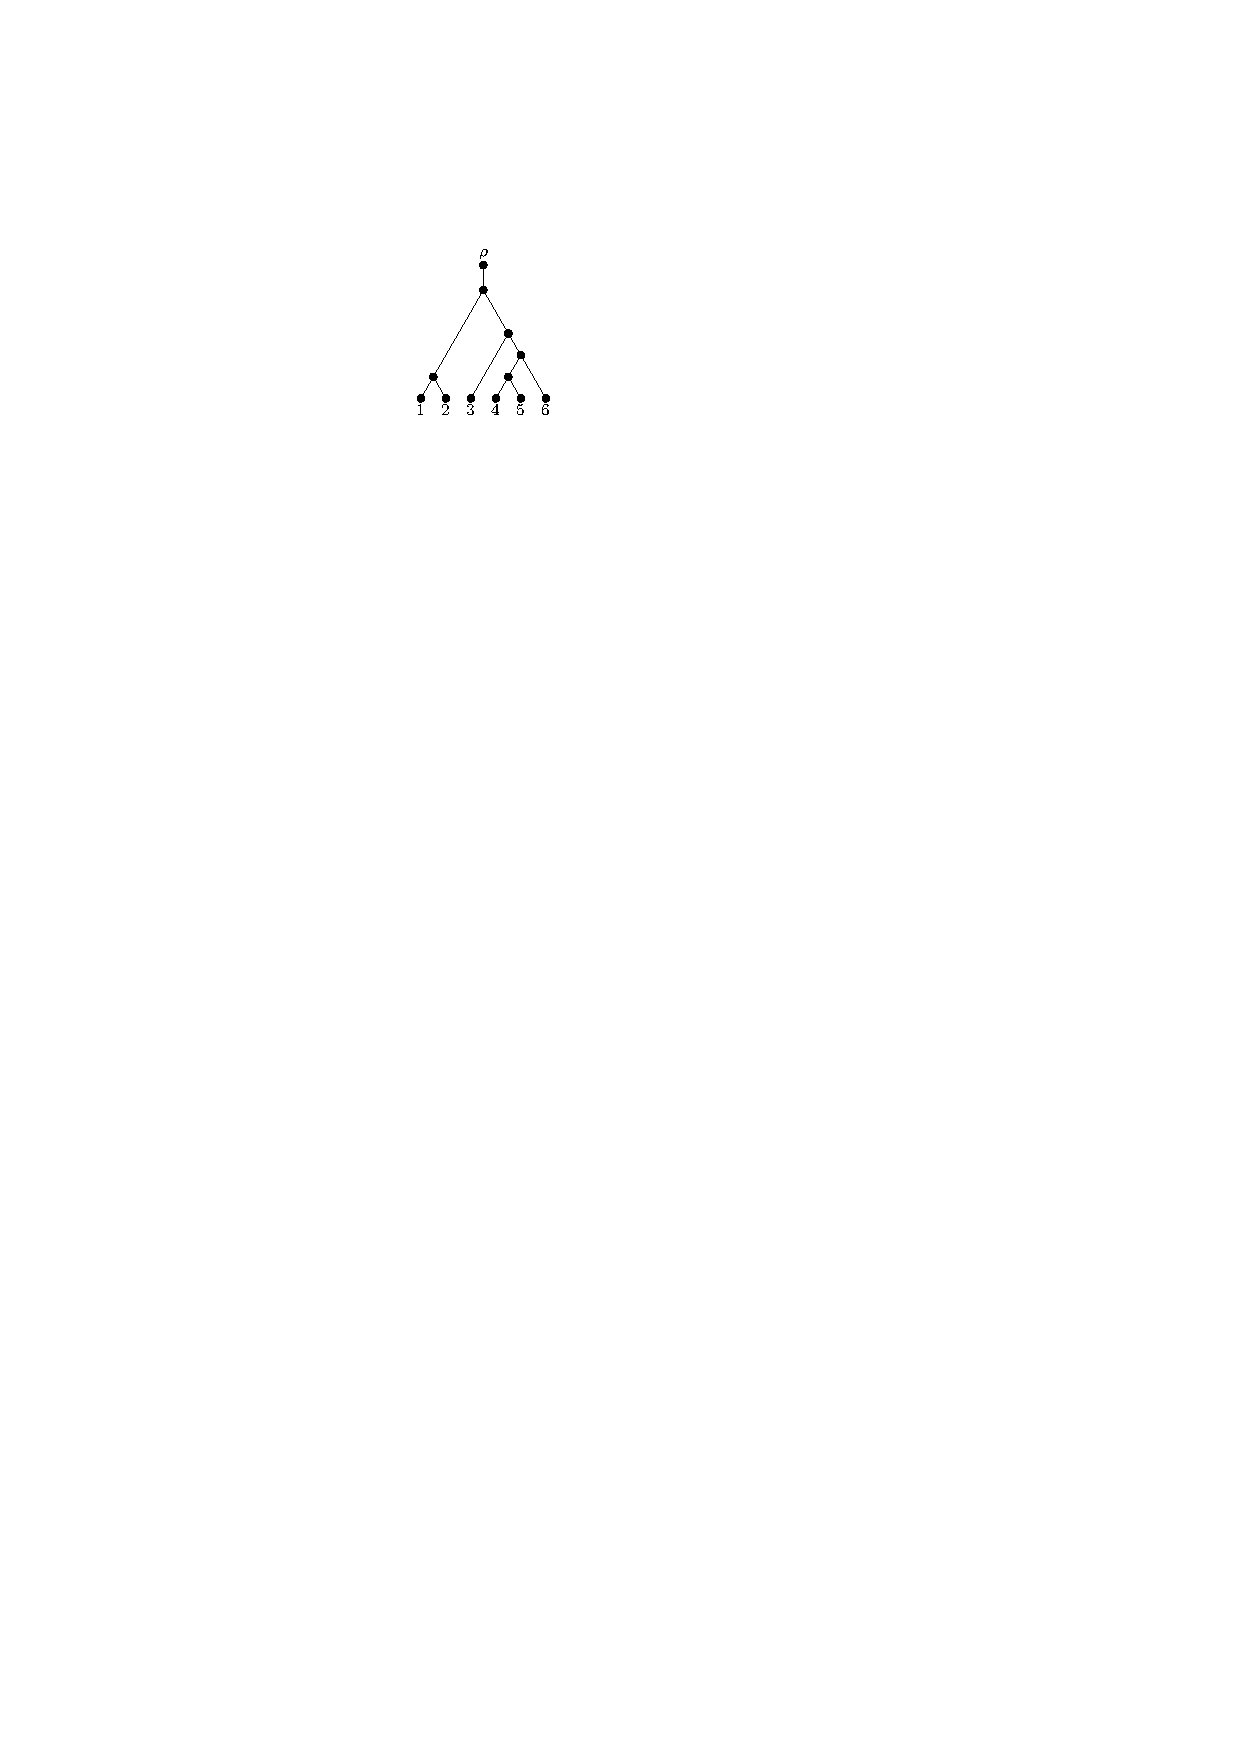
\includegraphics[scale=1.25]{figs/x-tree}}
	\hspace*{\stretch{2}}
	\subfigure[\label{fig:subtree}]{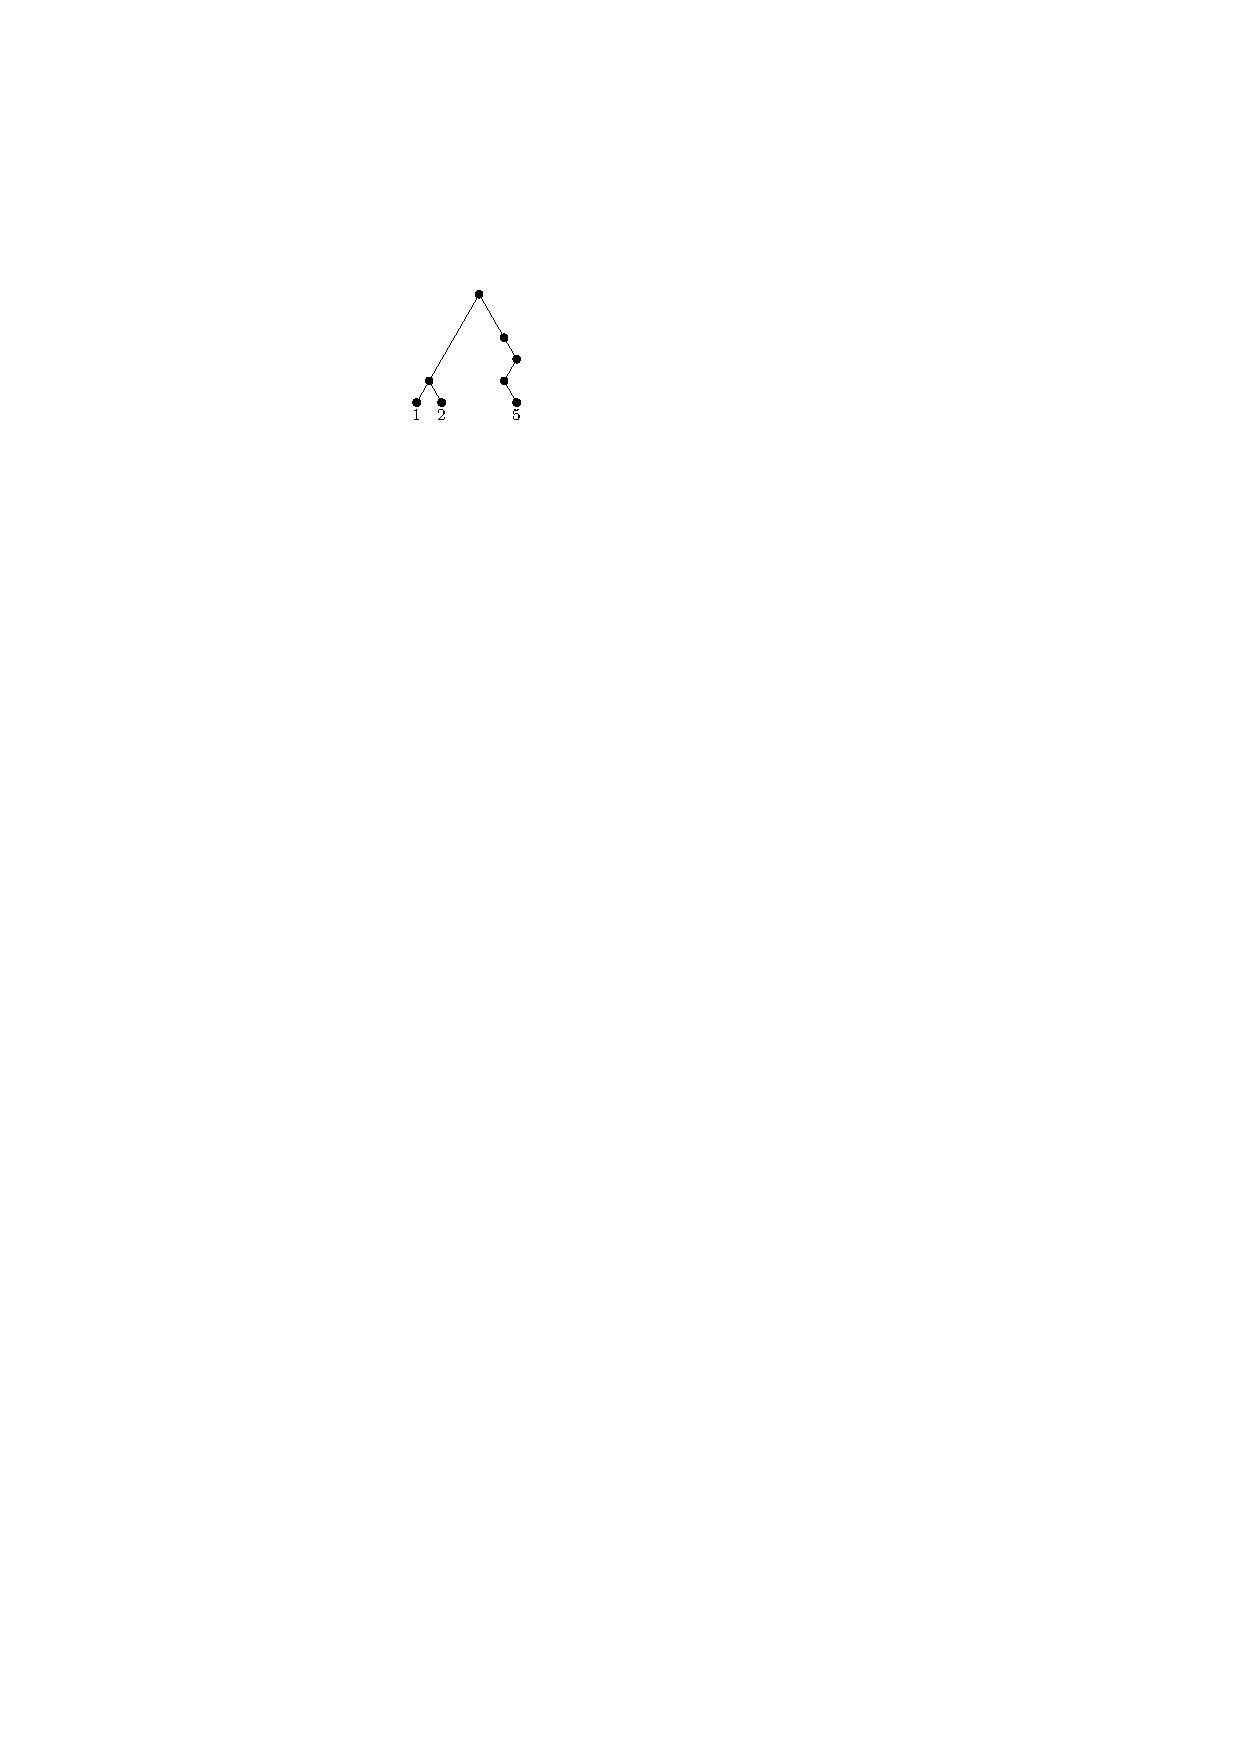
\includegraphics[scale=1.25]{figs/subtree}}
	\hspace*{\stretch{2}}
	\subfigure[\label{fig:induced}]{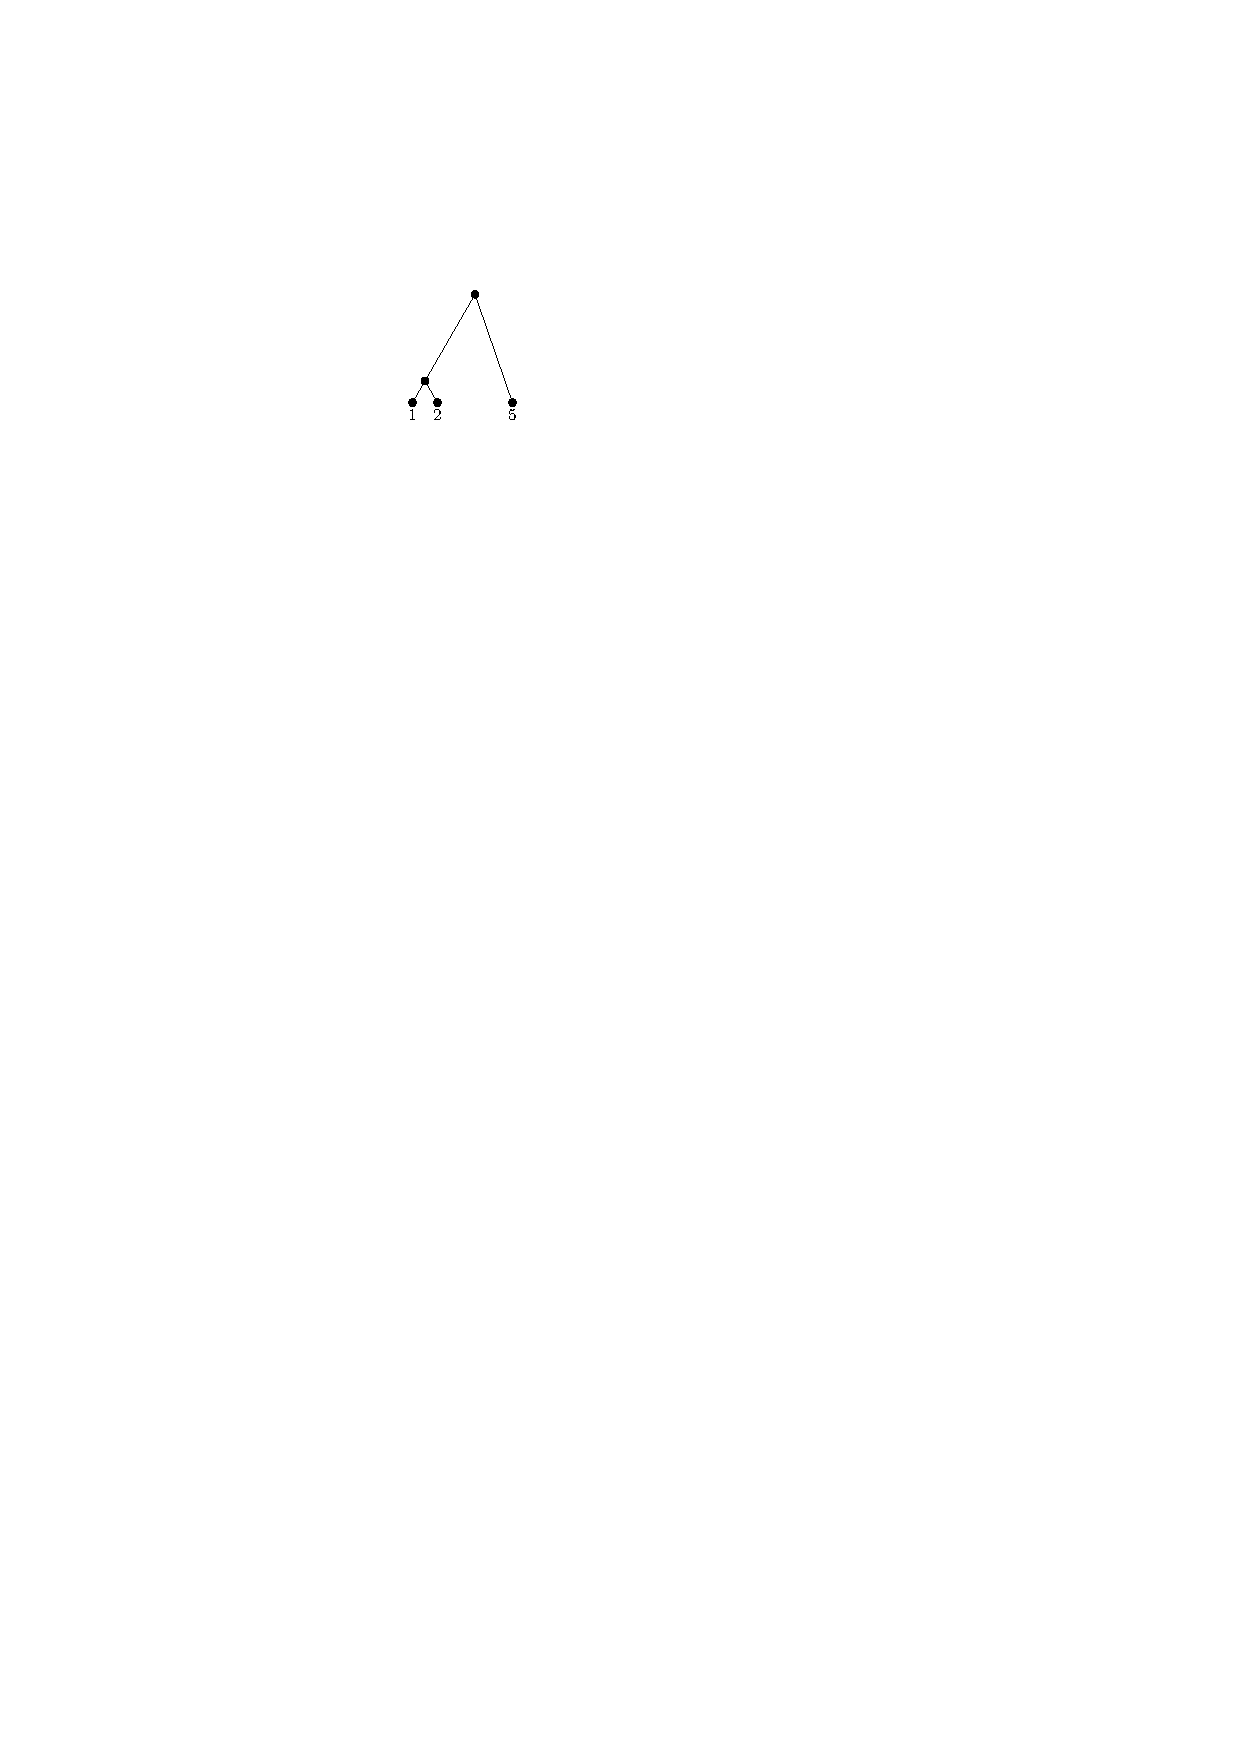
\includegraphics[scale=1.25]{figs/contracted-subtree}}
	\hspace*{\stretch{1}}
	\\
	\hspace*{\stretch{1}}
	\subfigure[\label{fig:spr}]{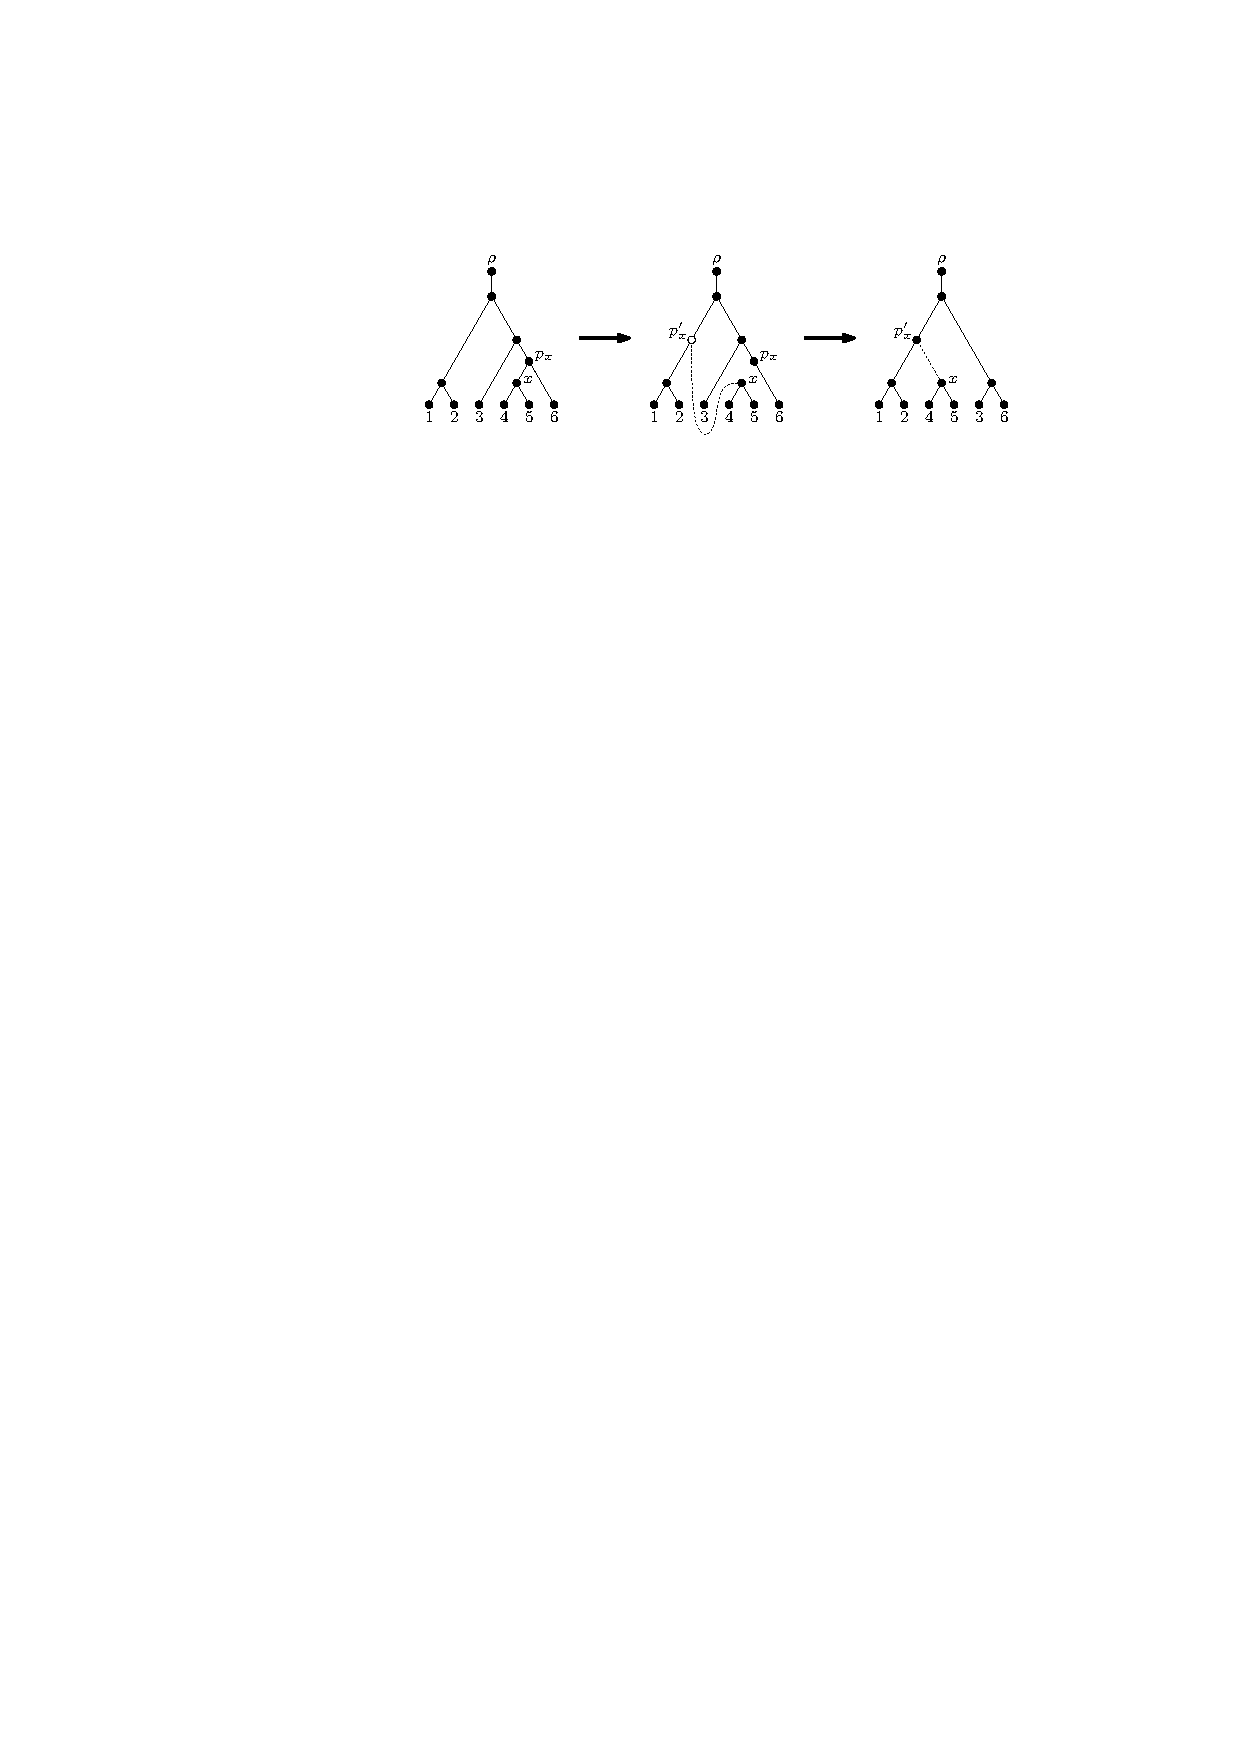
\includegraphics[scale=1.25]{figs/spr}}
	\hspace*{\stretch{1}}
	\\
	\hspace*{\stretch{1}}
	\hspace*{\stretch{1}}

	\caption{(a) An $X$-tree $T$.
		(b) $T(V)$, where $V = \set{1,2,5}$.
		(c) $T|V$.
		(d) An SPR operation transforms $T$ into a new tree $T'$ by \emph{pruning} a \emph{subtree} and \emph{regrafting} it in another location.}
	}
	\label{fig:trees}
\end{figure}
\begin{figure}
	\hspace*{\stretch{1}}
	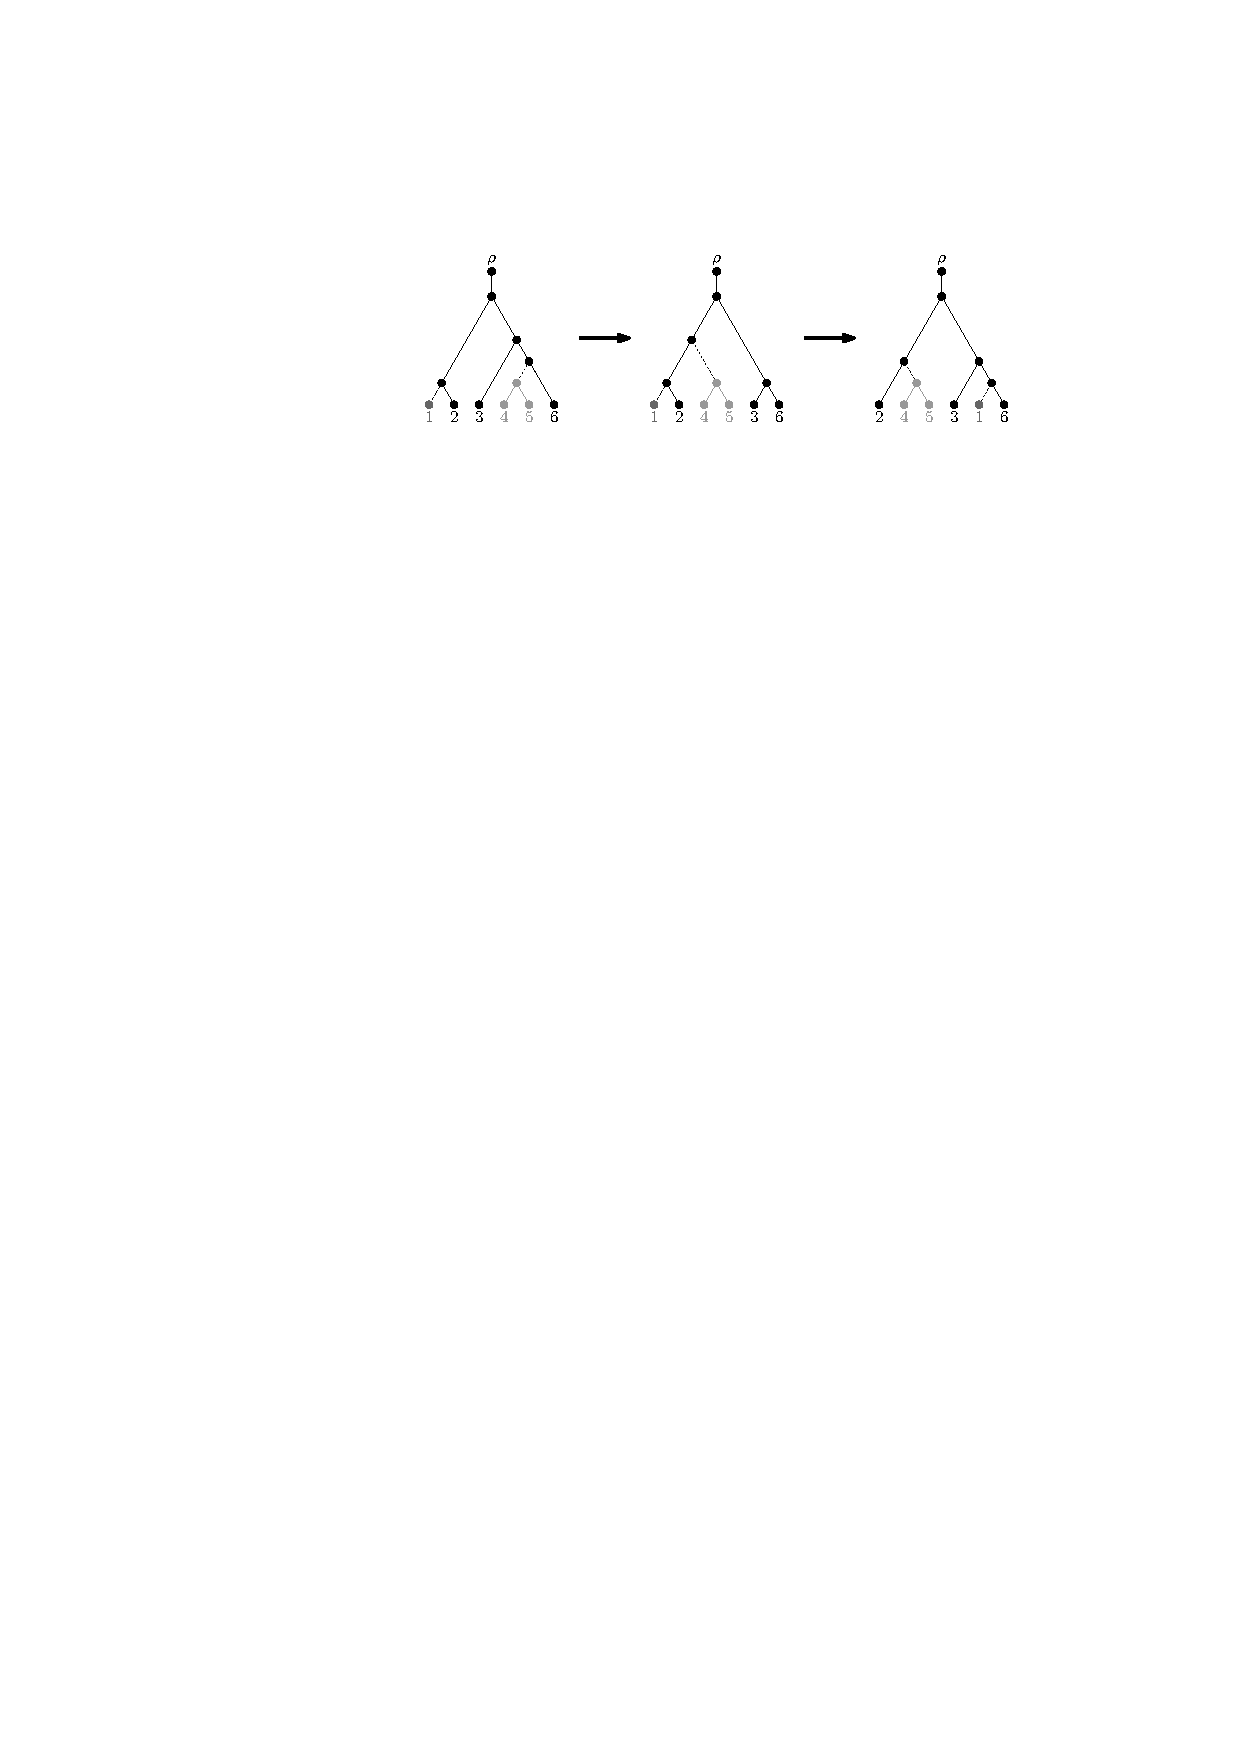
\includegraphics[scale=1.25]{figs/two-spr}
	\hspace*{\stretch{1}}
	\caption{Two trees differing by two SPR operations that move the grey subtrees.}
	\label{fig:two-spr}
\end{figure}
\begin{figure}
	\hspace*{\stretch{1}}
	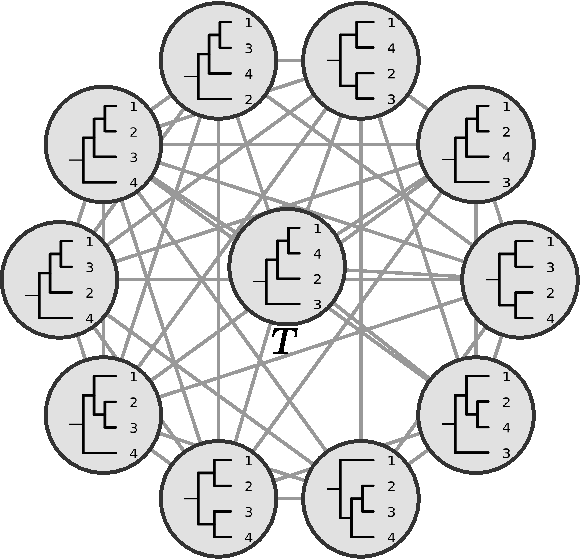
\includegraphics[width=0.6\textwidth]{figs/neighborhood}
	\hspace*{\stretch{1}}
	\caption{The neighborhood of an $X$-tree $T$ with 4 leaves, showing connections between neighbors.}
	\label{fig:neighborhood}
\end{figure}

We follow the definitions and notation from~\cite{bordewich05,whidden2013hybridization, Whidden2015-yi}.
A (rooted binary phylogenetic) $X$-tree is a rooted tree $T$ whose nodes have zero or two children.
Leaves of $T$ are bijectively labelled with the members of a label set $X$.
As in~\cite{bordewich05,whidden2013hybridization,Whidden2015-yi}, the tree is augmented with a labelled root node $\rho$ and $\rho$ is considered a member of $X$ (Fig.~\ref{fig:x-tree}).
We generally use $n$ to refer to the number of leaves in an $X$-tree.
For a subset $V$ of $X$, $T(V)$ is the smallest subtree of $T$ that connects all nodes in $V$ (Fig.~\ref{fig:subtree}).
The $V$-tree induced by $T$ is the smallest tree $T|V$ that can be obtained from $T(V)$ by suppressing unlabelled nodes with fewer than two children (Fig.~\ref{fig:induced}).
For the rest of the paper, \textbf{we will assume that all phylogenetic trees are rooted,} and thus that tree inclusion is rooted tree inclusion.
\todo{Figure of restriction and SPR operation}

A \emph{parent (sub)tree} of a subtree $U$ is the smallest subtree strictly containing $U$.
A \emph{parent edge} of a subtree $U$ is the edge connecting $U$ to the rest of the tree.
The \emph{internal edges} of a tree are the edges that do not contact a leaf (we do not consider a rooted tree to have a ``root edge'', so trees have a degree two root). \todo{Generally we add a $\rho$ label and root edge to make rSPR work formally. I've put this in the definition so lets see if this confuses anything.}
A \emph{ladder tree} (also known as a \emph{caterpillar tree}) is a tree such that every internal node has a leaf as a direct descendant.
A \emph{balanced tree} is a tree such that the sum of the depths of internal nodes is minimum over all trees with the same number of leaves.
The \emph{least common ancestor} (LCA) of a set $R$ of two or more nodes is the unique node that is an ancestor of each node $r \in R$ and at maximum depth.
Similarly, the LCA of two or more subtrees is the LCA of their parent nodes.

A \emph{subtree prune-and-regraft} (SPR) operation on an $X$-tree $T$ cuts an edge $e = (x, p_x)$ where $p_x$ denotes the parent of node $x$.
$T$ is divided into two subtrees $T_x$ and $T_{p_x}$ containing $x$ and $p_x$, respectively.
Then the operation adds a new node $p'_x$ to $T_{p_x}$ by subdividing an edge of $T_{p_x}$ and adding a new edge $(x, p'_x)$, making $x$ a child of $p'_x$.
Finally, $p_x$ is suppressed.
See Figure~\ref{fig:spr} for an example.
Note that the inclusion of $\rho$ allows for SPR moves that move subtrees to the root of the tree.\todo{Erm? I thought that we weren't going to have a root edge.}

SPR operations give rise to a distance measure between $X$-trees: $\dspr{T_1, T_2}$ is the minimum number of SPR operations required to transform an $X$-tree $T_1$ into $T_2$.
For example, the trees in Figure~\ref{fig:two-spr} are separated by two SPR operations.
Moreover, SPR operations naturally give rise to a graph on the set of $X$-trees.
Let $\mathcal{T}_n$ be the set of trees with $n$ leaves and label set $X = \set{1, 2, \ldots n, \rho}$.\todo{$\rho$ again?}
Then the SPR graph $G$ of $\mathcal{T}_n$ is the graph with vertex set $V(G) = \mathcal{T}_n$ and edge set $E(G) = \set{(T,S) \mid \dspr{T,S} = 1, T \in V, S \in V}$.
Observe that distances in this graph are given by $\dspr{\cdot,\cdot}$.

To avoid confusion between the two types of graph structures considered here, we refer to vertices of the SPR graph as \emph{vertices} and vertices of individual trees as \emph{nodes}.
Let $N(T)$ be the set of SPR neighbors of a tree $T$ (this does not include $T$).
For example, the tree with 4 leaves in Figure~\ref{fig:neighborhood} has 10 neighbors.
We say that the degree of $T$ is $\degree{T}$, that is, the number of trees which can be obtained from $T$ by a single SPR operation.
Because we assume that all trees are bifurcating, we use degree to refer only to the degree of SPR graph vertices.

Ollivier-Ricci curvature provides an intuitive formalization for quantifying the shape of a graph with respect to a random walk (or indeed any metric space, see~\cite{Ollivier2009-bw}).
Let $m_x$ and $m_y$ be probability densities of a specified random walk starting at points $x$ and $y$ of a graph $G = (V,E)$, respectively.
The $L^1$ transportation, or Wasserstein, distance between $m_x$ and $m_y$ is the minimum amount of ``work'' required to move $m_x$ to $m_y$ following the graph, that is
 $$ W_1(m_x, m_y) := \min_{\xi \in \Pi(m_x, m_y)} \sum \dspr{x,y} \xi(x,y),$$
where $\Pi(m_x, m_y)$ is the set of of assignments of probability from $m_x$ to pairs of vertices in $V \times V$. \todo{I tried to keep this simple, feel free to change.}

The curvature of $x$ and $y$ is then defined as:
\begin{equation}
\curvature{x, y} := 1 - \frac{W_1(m_x, m_y)}{d(x, y)}
\label{eq:curvatureDef}
\end{equation}
Positive curvature implies that $m_x$ and $m_y$ are ``closer'' than $x$ and $y$, zero curvature implies that they are neither closer nor farther, and negative curvature implies that $m_x$ and $m_y$ are on average more distant than $x$ and $y$.
Curvature thus provides an intuitive measure of the difficulty of moving between regions of the graph with the given random walk.


\section{Access times of random walks on the rSPR graph can be understood using distance, degree, and curvature}

\subsection{Computing rSPR treespaces}
\label{sec:computing_treespace}

We computed the rSPR treespaces for four to seven leaves.
This required a fast new algorithm for SPR graph construction, reducing the time required to do so from $\OhOf{m^2 n}$ to $\OhOf{mn^3}$, where $m$ is the number of trees in the graph ($(2n-3)!!$ in this case) and $n$ the number of leaves.
In previous work~\cite{Whidden2015-yi}, we constructed (unrooted) SPR graphs from subsets of $m$ high probability trees sampled from phylogenetic posteriors to compare mixing and identify graph effects.
Although the SPR distance (rooted and unrooted) is NP-hard to compute~\cite{bordewich05,hickey2008sdc}, it is fixed-parameter tractable with respect to the distance in the rooted case~\cite{bordewich05}.
In particular, one can determine in $\OhOf{n}$-time whether two rooted phylogenetic trees are adjacent in the SPR graph ($\OhOf{n^2}$-time for unrooted trees) using the algorithms of Whidden et al.~\cite{whidden2009unifying,whidden2010fast, whidden2013hybridization,Whidden2015-yi}.
We applied this method comparing each of the $m$ trees pairwise to identify adjacencies, requiring a total of $\OhOf{m^2n}$-time ($\OhOf{m^2n^2}$-time in the unrooted case).
However, applying this method to complete SPR graphs, with the $\OhOf{m^2}$ factor where $m = (2n-3)!!$, requires an enormous amount of computation.

To quickly compute dense SPR graphs (those containing a significant portion of the full treespace) we can avoid pairwise computations by successively adding trees to the graph:
\begin{enumerate}[label={\arabic*}.]
	\item Let $G$ be an empty graph
	\item For each of the $m$ trees in a specified but arbitrary order,
		\begin{enumerate}
			\item Add a vertex $i$ to the graph representing the current tree $T$ where $i$ is $T$'s order index
			\item For each of the $\OhOf{n^2}$ neighbors of $T$
				\begin{enumerate}
					\item If the current neighbor $S$'s index is in $G$ then add an edge $(j,i)$ to the graph, where $j$ is $S$'s order index
				\end{enumerate}
		\end{enumerate}
\end{enumerate}

\begin{theorem}
	\label{thm:construct_graph}
	The subgraph of the rSPR graph induced by a set $\mathcal{T}$ of $m$ trees with $n$ leaves can be constructed in $\OhOf{mn^3}$-time.
\end{theorem}
\begin{proof}
	We implement the graph as an adjacency list with integer-labelled vertices.
	As described above, the integer labels are simply the order of the input trees.
	Adding the vertices to the graph requires $\OhOf{m}$-time, as they are added in ascending order to the end of the vertex list.
	Adding the $\OhOf{mn^2}$ edges to the graph requires $\OhOf{mn^2 \log n}$-time (as the vertex degrees are $\OhOf{n^2}$).
	Enumerating the neighbors of $T$ requires $\OhOf{n^3}$-time for each $T$, for a total of $\OhOf{mn^3}$-time.
	We discuss below, in Section~\ref{sec:random_walks} how to do so efficiently without considering duplicate neighbors.
	We store the tree to index mappings for current vertices of $G$ in a trie using the $\OhOf{n}$-length Newick representation of the tree.
	These representations are made unique by ordering the tree so that leftmost subtrees contain the smallest alphanumeric label of descendants.
	This requires only $\OhOf{n}$-time for each tree (i.e. a total of $\OhOf{mn^3}$-time) using a standard nodes and pointers representation of the tree and assuming integer leaf labels (a simple $\OhOf{mn\log n}$ leaf preprocessing step could be applied to extend this procedure to realistic phylogenetic trees).
	Similarly, it takes $\OhOf{n}$-time to determine the index of each of the $\OhOf{mn^2}$ $S$'s.
	Therefore the graph can be constructed in $\OhOf{mn^3}$-time.
\end{proof}
This procedure has been implemented in the C++ program \texttt{dense\_spr\_graph} of the software package \texttt{spr\_neighbors}~\cite{spr_neighbors}, which outputs an edge list format graph suitable for input to other software.
Our fast graph construction procedure reduced the time required to compute the 10,395-vertex 7-taxon rSPR tree space from 2,104.68 seconds to 12.71 seconds on an Intel Core 2 Duo E7500 desktop running Ubuntu 14.04.
Moreover, although we do not study the 135,135-vertex 8-taxon tree space in this paper, our algorithm required only 303.45 seconds to construct it.
Constructing the 8-taxon tree space using the previous method required 377,395 seconds (more than 4 days), and that method is infeasible for constructing larger tree spaces.
Thus, we believe this fast graph construction procedure will itself be useful for further studies of treespace subsets similar to~\cite{Whidden2015-yi}.

\subsection{Computing curvature values}
We computed all of the curvatures for pairs of trees with up to seven leaves to gain an intuitive understanding of the distribution of curvatures.
We first used \texttt{dense\_spr\_graph} to compute the rSPR treespaces for four to seven leaves, as discussed in Section~\ref{sec:computing_treespace}.
We then compute curvatures for given pairs of trees directly, by using linear programming to compute the minimal mass transport $W_1$ using the SAGE \cite{SAGE} front-end to the GLPK \todo{GLPK} solver; code can be found in \cite{gricci}.

This would have required an enormous amount of computation to directly compute curvatures for the $((2n-3)!!)^2$ pairs of trees with $n$ leaves.
We instead exploited the fact that pairs of trees which are equivalent modulo label renumbering are symmetric in the rSPR graph and therefore guaranteed to have the same curvature.
We thus directly computed curvature values for one representative pair from each such equivalence class, or \emph{tanglegram} \cite{Venkatachalam2010-zh}; the enumeration methods are described in a manuscript in preparation, and the SAGE \cite{SAGE} and GAP4 \cite{GAP4} code can be found online \cite{tangle}.


\subsection{Simulating random walks on the rSPR graph}
\label{sec:random_walks}
We next explored the correspondence between curvature and graph effects.
To do so, we first simulated Metropolis-Hastings random walks on the rSPR graphs with up to seven leaves.
The uniform random walk moves from the current vertex to one of its neighbors uniformly at random.
However, this makes the walk more likely to sample higher degree vertices.
In contrast, the Metropolis Hastings (MH) random walk with constant likelihood function proposes a move from a tree $T$ to a neighbor tree $S$ uniformly at random and then accepts the move according to the Hastings ratio, $\min\left(1, \frac{\degree{T}}{\degree{S}}\right)$.
The MH random walk is guaranteed to sample each tree uniformly at random and is therefore representative of a phylogenetic MCMC program sampling trees under a uniform prior.

To efficiently simulate the MH random walk, we developed a linear-time algorithm for proposing SPR moves that does not require the rSPR graph to be explicitly built and stored in memory.
A na\"ive approach would require $\OhOf{n^3}$ time---$\OhOf{n}$ time to generate each of the $\OhOf{n^2}$ neighbors of a given tree---and then one could be picked uniformly at random.
To eliminate an $\OhOf{n^2}$ factor, we developed a deterministic ordering of SPR moves with a one-to-one correspondence to SPR neighbors, as described in the next paragraph.
Given such an order, a uniform neighbor can be selected by its index in $\OhOf{n}$ time.
We note that the recursive formula of Song~\cite{Song2003-gf} for the degree of a tree does not group SPR moves that move a particular subtree, and thus would still require $\OhOf{n^2}$ time to select a specific SPR neighbor by index.

Instead, we consider the distribution of SPR moves in terms of the number of nodes contained within a subtree.
Recall that a tree with $n$ leaves has $2n-1$ total nodes.
Given a subtree $R$ with $x$ nodes, observe that there are $2n-1 - x$ possible locations to regraft $R$.
However, some of these moves will result in the same neighboring tree as other SPR moves.
In particular, where a node's edge means the edge connecting the subtree rooted at that node to the rest of the tree:
\begin{enumerate}
\item Moving $R$ to its sibling edge results in the same tree, not a neighboring tree,
\item Moving $R$ to its parent edge results in the same tree,
\item Moving $R$ to its grandparent edge is the same as moving its aunt to its sibling edge
\item Moving $R$ to its aunt edge is the same as moving its aunt to $R$'s edge.
\end{enumerate}
We can thus assign $2n-1-x-4$ moves to any node at a depth greater than 1 and $2n-1-x-2$ moves to depth 1 nodes (lacking both an aunt and grandparent).
Call the portion of the neighborhood of a tree $T$ that can be obtained by moving a subtree $R$ rooted at a node $u$, and that is assigned to $u$, $N(T,u)$.
In this manner, we achieve an alternative solution for computing the degree of a tree in the SPR graph:

\begin{lemma}
	\label{lem:compute_degree}
	For a tree $T$ with $n$ leaves,
	$$\degree{T} = \sum_{u \in T} \size{N(T,u)},$$
	for nodes $u$ of $T$, where $N(T,u)$ is as defined above, and:
	$$\size{N(T,u)} = \begin{cases}
		2n - 1 - x - 4 &\text{if depth($u$) $ > 1$, } \\
		2n - 1 - x - 2 &\text{if depth($u$) $ = 1$ } \\
		0 &\text{if depth($u$) $ = 0$ } \\
	\end{cases}.$$
	Moreover, each tree of $N(T,u)$ can be obtained by an SPR operation that moves the subtree rooted at $u$.
\end{lemma}
\begin{proof}
	The statement follows if each of the neighbor assignments are disjoint, that is $N(T,u) \cap N(T,v) = \emptyset$, for all nodes $u$, $v$ of $T$.
	So, suppose, for the purpose of obtaining a contradiction, that there exist two nodes $u$ and $v$ of $T$ such that there exists a tree $S \in (N(T,u) \cap N(T,v))$.
	Then $S$ can be obtained from $T$ by moving the subtrees rooted at $u$ or $v$.
	Call these $U$ and $V$, respectively.
	This implies that both $T \setminus U = S \setminus U$ and $T \setminus V = S \setminus V$.
	Then the SPR moves that move $U$ or $V$ to obtain $S$ must be nearest neighbor interchanges (NNIs), that is SPR moves which move their subtree to one of four locations: their grandparent edge, aunt edge, sibling's left child edge or sibling's right child edge.
	This implies that, without loss of generality, $U$ is moved to its grandparent edge and $V$ to $U's$ sibling (i.e. (iii) above) or $U$ is moved to its aunt edge and $V$ to $U$'s edge (i.e. iv above), a contradiction.
	Therefore the claim holds.
\end{proof}


In particular, this formulation groups moves that move the same subtree.
We can thus apply the following algorithm to select a neighbor uniformly at random for a tree $T$:

\begin{enumerate}[label={\arabic*}.]
	\item	compute the degree of $T$, $\degree{T}$.
	\item pick a random integer $r$ in the range $[1,\degree{T}]$
	\item label each node $u$ of $T$ by its preorder number and compute the number of nodes in the subtree rooted at each $u$.
\item for each tree node $u$ and while $r > 0$
	\begin{enumerate}
		\item decrease $r$ by $\size{N(T,u)}$
		\item if $r < 0$, let $S$ be the $\abs{r}$ member of $N(T,u)$ and terminate the for loop
	\end{enumerate}
\item return the neighbor $S$
\end{enumerate}

\begin{lemma}
	\label{lem:select_random_neighbor}
	Given a tree $T$, an SPR neighbor of $T$ can be chosen uniformly at random in $\OhOf{n}$-time using $\OhOf{n}$ space.
\end{lemma}
\begin{proof}
	We apply the above procedure.
	We use a standard nodes and pointer representation of the trees, which can be constructed in $\OhOf{n}$-time from a newick string representation and uses linear space in $n$.
	We can compute the degree of $T$ in linear time and space using Lemma~\ref{lem:compute_degree}.
	To efficiently compute $\size{N(T,u)}$ for each node $u$ of $T$, we require the number of nodes $x$ in the subtree rooted at $u$.
	We precompute these by (1) labeling each node with its preorder number in a preorder traversal and (2) summing the number of descendant nodes in a postorder traversal and storing the results in an array indexed by preorder number.
	Both of these traversals require $\OhOf{n}$-time.
	There are $2n-1$ = $\OhOf{n}$ nodes of $T$, and $\size{N(T,u)}$ can be computed in constant time using the subtree sizes.
	Moreover, the tree $S$ can be found by iterating over the edges of $T$ that are not contained within $u$'s subtree to select the corresponding SPR destination.
	Finally, we require linear time to apply the chosen SPR operation which entails removing a node, adding a node, and updating a constant number of pointers.
	Thus, the for loop requires linear time.
	By Lemma~\ref{lem:compute_degree} the chosen tree is an SPR neighbor of $T$ and is chosen uniformly at random.
	Therefore, the procedure uses linear time and space and selects an SPR neighbor of $T$ uniformly at random.
\end{proof}

Observe that this procedure can be easily adapted to explore the full neighborhood of a tree in $\OhOf{n^3}$ time, which we use for Theorem~\ref{thm:construct_graph}.
We thus have the following corollary:

\begin{corollary}
	Given a tree $T$, the SPR neighbors of $T$ can be enumerated in $\OhOf{n^3}$-time.
\end{corollary}

We implemented this procedure in the C++ package \texttt{random\_spr\_walk}~\cite{random_spr_walk}.
We sampled \ldots \todo{sampling and runtime information}.

\cite{GAP4}

\subsection{Access time computation}

The access time for a pair of vertices in a graph is the (random) number of iterations required to go from one of the vertices to the other in a random walk~\cite{lovasz1993random}; we were interested in the connection between curvature and access time.
In previous work, we computed mean access times (MAT) between pairs of trees in the MCMC random walks---the mean number of iterations required to move from one tree to the other.
We applied this work to demonstrate graph effects in uSPR subgraphs of real MCMC samples using MrBayes~\cite{Whidden2015-yi} using the \texttt{sprspace}~\cite{sprspace} software.

Here, to gain more insight, we used simulation to approximate the entire access time distribution.
As before, calculating these distributions for all pairs of trees would have required a tremendous amount of memory and computational power in order to get good estimates.
Here again we use the insight that the access time for a pair of trees with a simple random walk does not depend on the actual labeling of those trees, but rather only on their relative labeling.
Thus rather than enumerate access times between trees, we enumerate times between pairs of trees in a tanglegram.
For example, because the pairs
$\{(((1,2),3),4) ((1,2),(3,4))\}$ and
$\{(((1,4),3),4) ((1,4),(2,3))\}$
are the same after relabeling, their access times will have identical distributions.
Thus to calculate the empirical distributions of access times we aggregate all access times for the same tangle.


\subsection{Results}

After the chain has achieved stationarity, one sees a


\section{Rooted SPR Neighborhoods}

In the absence of a bias provided by a likelihood function, curvature for the random walks we consider is entirely determined by the degree of vertices in the graph.
Thus, in order to provide bounds on curvature, we will begin by bounding differences between degrees.

\begin{lemma}[{Song~\cite{Song2003-gf}}]
    \pushQED{\qed}
	\label{lem:degree_extremes}
	Let $T$ be a rooted phylogenetic tree with $n$ leaves. Then
	\begin{enumerate}
		\item $\degree{T} = 3n^2 - 13n + 14$, if $T$ is a ladder tree,
		\item $\degree{T} = 4(n-2)^2 - 2 \sum_{m=1}^{n-2} \floor{\log_2(m+1)}$, if $T$ is a balanced tree, and
		\item  $3n^2 - 13n + 14 \le \degree{T} \le 4(n-2)^2 - 2 \sum_{m=1}^{n-2} \floor{\log_2(m+1)}$, otherwise.
	\end{enumerate}
    \popQED
\end{lemma}

We now bound the relative and exact difference in SPR degree between two trees with $n$ leaves.

\begin{lemma}
	\label{lem:degree_max_delta}
	Let $T$ and $S$ be rooted phylogenetic trees with $n \ge 3$ leaves, and assume without loss of generality that $\degree{T} \le \degree{S}$.
	Then:
	\begin{enumerate}
		\item $\frac{\degree{T}}{\degree{S}} \ge \frac{3}{4}$, and
		\item $\degree{S} - \degree{T} \le n^2 - 5n + 6$.
	\end{enumerate}
\end{lemma}
\begin{proof}
	To prove (i), we simply note from Lemma~\ref{lem:degree_extremes} that the ladder tree achieves the minimum degree, and the balanced tree achieves the maximum degree:
	\begin{align*}
		\frac{\degree{T}}{\degree{S}} \ge\ &\frac{3n^2 - 13n + 14}{4(n-2)^2 - 2 \sum_{m=1}^{n-2} \floor{\log_2(m+1)}} \\
		\ge\ &\frac{3n^2 - 13n + 12}{4(n-2)^2 - 2(n-2)} \\
		\cuttable{= \ &\frac{3n^2 - 13n + 12}{4n^2 - 16n + 16 - 2(n-2)} \\}
		= \ &\frac{3n^2 - 13n + 12}{4n^2 - 18n + 20} \\
		\cuttable{\ge\ &\frac{3n^2 - 13n + 12}{4n^2 - 17\frac{1}{3}n + 18} &\forall n \ge 3 \\}
	\end{align*}
	which is greater than 3/4 when $n \ge 3$.
    Similarly for (ii):
	\begin{align*}
		\cuttable{\degree{S} - \degree{T}
		\le\ &(4(n-2)^2 - 2 \sum_{m=1}^{n-2} \floor{\log_2(m+1)})
		- (3n^2 - 13n + 14) \\}
		\le\ &(4(n-2)^2 - 2(n-2)) - (3n^2 - 13n + 14) \\
		\cuttable{=\ &4n^2 - 16n + 16 - 2n +4 - 3n^2 + 13n - 14 \\}
		=\ &n^2 - 5n + 6.
	\end{align*}
\end{proof}

We can improve these bounds in the case of adjacent trees.
To do so, we require the following lemma that characterizes exactly how the degree of a tree changes after an rSPR operation.

\begin{lemma}
\label{lem:degree_change}
Let $T$ and $S$ be phylogenetic trees such that $S$ can be obtained from $T$ by moving a subtree $R$ with $k$ leaves from its position adjacent to subtree $U$ to a location adjacent to subtree $V$.
Let $L$ be the $\lca{U,V}$ in $T$.
Let $a$ be the number of intermediate nodes on the path from the parent of $R$ to $L$ in $T$, excluding endpoints.
Similarly, let $b$ be the number of intermediate nodes on the path from $V$ to $L$ in $T$, excluding endpoints.
Let $i$ be the number of leaves in $U$ and $j$ be the number of leaves in $V$, excluding any leaves of $R$.
Then the degrees of $T$ and $S$ differ by:
$$2\left(k(a-b) + i - j\right).$$

\end{lemma}
\begin{proof}
The set of permissible SPR moves changes in four different ways due to the movement of $R$:
(i) subtrees that include nodes on the path from $U$ to $L$ may now be moved into $R$ and its newly introduced parent node,
(ii) subtrees that include nodes on the path from $V$ to $L$ may no longer be moved into $R$ and its parent node,
(iii) $R$'s parent subtree may now be moved into $U$, and
(iv) $R$'s parent subtree may no longer be moved into $V$.
No additional moves are introduced or blocked by the original SPR operation on $R$.

Recall that a rooted tree with $k$ leaves has $2(k-1)$ internal edges (recall that we are excluding any ``root edge'' in these calculations).
In the first case there are $a$ subtrees that can now be moved onto the $2k$ edges in $R$ (including its newly introduced parent edge and one of the newly subdivided root edges of $V$) for a total gain of $2ka$ distinct moves.
Similarly, we lose $2kb$ moves in the second case.
In the third case, $R$'s parent subtree may now make $2(i-1)$ moves into $U$.
Similarly, we lose $2(j-1)$ moves in the fourth case.

The difference in SPR degree is thus $2ka - 2kb + 2(i-1) - 2(j-1)$ as claimed.
\end{proof}

Moreover, we can use these ideas to determine the number of SPR moves that are, in some respects, independent of a given SPR move.
That is, for two trees $S$ and $T$ differing by a single SPR move, we wish to know the number of SPR moves that are applicable to both trees rather than unique to one of the trees.
To formalize this concept, we consider pairs of trees $T' \in N(T)$ and $S' \in S(T)$ such that $\dspr{T',S'} = 1$.
The number of such ``squares'' involving two adjacent trees will play a key rule in our bounds on curvature, as they push the curvature of those trees towards 0.

\begin{corollary}
\label{cor:paired_neighbors}
Continuing with the setting and notation in Lemma~\ref{lem:degree_change}, at least
$$o := \deg(T) - 2kb - 2(j-1) = \deg(S) - 2ka - 2(i-1)$$
trees in the neighborhood of $T$ can be paired with $o$ trees in the neighborhood of $S$ such that the pairings are disjoint and $\dspr{T',S'} = 1$ for each $(T',S')$ pair.
\end{corollary}
\begin{proof}
By the same arguments as in the proof of Lemma~\ref{lem:degree_change}, $o$ SPR moves can be applied to $T$ and $S$ with the same source and target nodes.
For each such $(T',S')$ pair, we can move $R$ in either tree to obtain the other member of the pair.
\end{proof}

We can now use Lemma~\ref{lem:degree_change} to improve the bounds in Lemma~\ref{lem:degree_max_delta} for the case of two adjacent trees.
\begin{lemma}
	\label{lem:degree_max_delta_adjacent}
	Let $T$ and $S$ be rooted phylogenetic trees with $n \ge 3$ leaves, such that $\degree{T} \le \degree{S}$ and $\dspr{T,S} = 1$.
	Then:
	\begin{enumerate}
		\item $\degree{S} - \degree{T} \le 2\floor{\frac{n-2}{2}}\ceil{\frac{n-2}{2}} \le \frac{1}{2} (n-2)^2 $.
		\item $\frac{\degree{T}}{\degree{S}} \ge \frac{5}{6}$, $\forall n \ge 4$, and
		\item $\lim_{n\rightarrow\infty}\frac{\degree{T}}{\degree{S}} =  \frac{6}{7}$.
	\end{enumerate}
\end{lemma}
\begin{proof}
	We first prove (i).
	By Lemma~\ref{lem:degree_change}, $\degree{S} - \degree{T} = 2(k(a-b) + i - j)$.
	This value is maximized by making $L$ the root and minimizing $b$, namely by setting $b=0$.
	The resulting equation $2(ka + i - j)$ is similarly maximized by setting $i=1$ (which allows us to increase $a$) then maximally balancing the terms in the product $ka$ as follows.

	There are two cases, depending on whether the subtree of $k$ leaves is moved to the root or not.
    If not, then we set $j=1$ and split the remaining $n-b-i-j = n-2$ leaves between $k$ and $a$ in as balanced a way as possible, giving (i).
	Note that this corresponds to moving the bottom subtree of $\floor{\frac{n-2}{2}}$ or $\ceil{\frac{n-2}{2}}$ leaves in a ladder tree to the root-most leaf of the tree.

	If the subtree of $k$ leaves is moved to the root, then we do not need to exclude the target branch from $k$ and $a$, gaining an additional leaf to balance the product $ka$ at the cost of increasing $j$.
	This corresponds to moving the bottom subtree of $\floor{\frac{n}{2}}$ or $\ceil{\frac{n}{2}}$ leaves in a ladder tree to the root.
	Namely, we have $2(ka + 1 - j)$, where $j = n - k = a + 1$.
	If we move the additional leaf, we have:
$$\degree{S} - \degree{T} \le 2\left(\ceilXXL{\frac{n}{2}}\floorV{\frac{n-2}{2}}  + 1 - \left(\floorV{\frac{n-2}{2}} + 1\right)\right) = 2\floorV{\frac{n-2}{2}}\ceilV{\frac{n-2}{2}}$$
like before.
Similarly, if we do not move the additional leaf, we also have:
$$\degree{S} - \degree{T} \le 2 \left(\ceilV{\frac{n-2}{2}}\floorXXL{\frac{n}{2}} +1 -  \left(\ceilV{\frac{n-2}{2}} + 1\right)\right) = 2\floorV{\frac{n-2}{2}}\ceilV{\frac{n-2}{2}},$$
proving (i).

The relative change in degree, $\frac{\degree{T}}{\degree{S}}$, can also be written as $\frac{\degree{T}}{\degree{T} + (\degree{S} - \degree{T})}$.
By (i), we have that $\degree{S} - \degree{T} \le \frac{1}{2} (n-2)^2$,
so $\frac{\degree{T}}{\degree{S}} \ge \frac{\degree{T}}{\degree{T} + \frac{1}{2} (n-2)^2} $.
This bound is minimized when $\degree{T}$ is minimized, and recall by Lemma~\ref{lem:degree_extremes} that $\degree{T}$ is bounded below by $3n^2 - 13n + 14$.
	Thus
	\begin{align*}
		\frac{\degree{T}}{\degree{S}} &\ge \frac{3n^2 - 13n + 14}{3n^2 - 13n + 14 + \frac{1}{2}(n-2)^2} \\
		&\ge \frac{3n^2 - 13n + 14}{3.5n^2 - 15n + 16}.
	\end{align*}
	Statements (ii) and (iii) follow from this bound.
    % 3*16 - 13*4 + 14 = 10
    % 3.5*16 - 15*4 + 16 = 12

\end{proof}


Next, we bound the number of neighbors shared by two adjacent trees.
The number of such "triangles" involving two adjacent trees has a key role in determining whether the curvature of two adjacent trees is positive or negative.

\begin{lemma}
	\label{lem:shared_neighbors}
Let $T$ and $S$ be rooted $X$-trees such that $\dspr{T,S} = 1$.
Then $\size{N(T) \cap N(S)} \le 6n - 17$.
\end{lemma}

\begin{proof}
	$T$ and $S$ differ by one SPR move that moves a subtree $R$.
	Pick a neighbor $U \in N(T) \cap N(S)$ of both $T$ and $S$ (this intersection is not empty: $T$ and $S$ are different, so $R$ contains at most $n-2$ of the leaves, thus there must be at least one other tree $U$ obtained by moving $R$ in $T$ and $S$).
	Then either (i) $T$ and $U$ differ in the location of $R$, or (ii) $T$ and $U$ differ in the location of another subtree $Q$.
	In the latter case, $T|(X \setminus L(Q)) = S|(X \setminus L(Q))$ because $T$ and $S$ differ only in the location of $R$ and $\dspr{T,U} = \dspr{S,U} = 1$.
	Then leaves $r' \in R$, $q' \in Q$, and $u' \in U$, for some subtree $U$, form a triple of $T$ and a different triple in $S$.
	This incompatible triple can be resolved in at most $6n - 17$ ways, the maximum of which is reached when $Q$, $U$, and $R$ are themselves a ``triple'' of subtrees.
	By Lemma~\ref{lem:compute_degree}, each of the subtrees is assigned to at most $2n-6$ unique moves.
	Moreover, one additional overlapping move also moves one of the subtrees (that of the aunt of the LCA of the three subtrees).
	The number of shared neighbors is thus at most $3(2n-6) + 1 = 6n-17$.
	Note that this bound is tight when, for example, $T$ and $S$ are ladders with a different configuration of 3 leaves at maximum depth.
\end{proof}





\section{Curvature}
For the purposes of this paper, $\kappa_n$ is the Ricci-Ollivier curvature \eqref{eq:curvatureDef} on the $n$-taxon rSPR graph with respect to a specified random walk and $W_{1,n}$ is the corresponding mass transport term.

We first consider properties of the uniform random walk on the rSPR graph.
Assume that the random walk begins at a tree $T$.
The uniform random walk selects a tree uniformly at random from $N(T)$.
We denote the curvature of the uniform random walk between two trees $T$ and $S$ with $\curvature{T,S}$.
Recall that $\curvature{T, S} := 1 - \frac{W_1(m_T, m_S)}{d(T, S)}$.
For the uniform random walk, $m_T$ is simply the probability measure assigning a mass of $\frac{1}{\degree{T}}$ to each of the neighbors of $T$.

\begin{proposition}
Fix a positive integer $k$ and let $R$ be a tree with $k$ leaves.
Let $\{T_n \mid n > k\}$ be a sequence of phylogenetic trees all containing $R$, and let $\{S_n \mid n > k\}$ be the same sequence $T_n$ but with $R$ cut off and attached at a different location.
Then $\lim_{n \rightarrow \infty} \curvature{T_n,S_n} = 0$ for the uniform random walk on the SPR graph.
\end{proposition}
\begin{proof}
Because $d(T_n, S_n) = 1$, we will prove the proposition by showing that the mass transport term $W_{1,n}$ sits between two bounds, each of which has limit 1 as $n$ goes to infinity.

To start we demonstrate the proposition in the case that $T_n$ and $S_n$ have the same number of neighbors.
First we claim that $W_{1,n}$ is bounded above by $(\degree{T_n}+\OhOf{kn})/\degree{T_n}$ by exhibiting a mass transport program satisfying that bound.
Let $(T'_n, S'_n)$ be any of the $o$ pairs of neighbors of $(T_n, S_n)$ which are one SPR move apart as per Corollary~\ref{cor:paired_neighbors}.
We pair these trees in the mass transport.
There are $\OhOf{kn}$ trees unmatched by this pairing, and we can pair each of them arbitrarily with another tree of distance at most 3.
Thus, $W_{1,n}$ is bounded above by $(\degree{T_n} + \OhOf{kn}) / \degree{T_n}$.

A lower bound is also available because we can't do better than distance 1 for all trees except for shared neighbors, of which there are $\OhOf{n}$ by Lemma~\ref{lem:shared_neighbors}.
By ignoring these trees we get a lower bound of $(\degree{T_n} - (\OhOf{n}))/\degree{T_n}$ for $W_{1,n}$.

The desired control of $W_{1,n}$ is thus obtained because $\degree{T_n}$ is quadratic in $n$.

Now we prove the proposition when the number of neighbors differ.
Assume without loss of generality that $\degree{T_n} < \degree{S_n}$.
By Lemma~\ref{lem:degree_change}, $\degree{S_n} - \degree{T_n} = 2(k(a-b) + i - j)$, where each of $\{a,b,i,j\}$ is less than $n$.
Thus, $\degree{S_n} - \degree{T_n} = \OhOf{kn}$.
We again pair neighbor $T'_n$ of $T$ with neighbor $S'_n$ of $S$ such that $\dspr{T'_n, S'_n}=1$ but, as $\degree{T_n} < \degree{S_n}$ we can only account for at most $\degree{T_n} / \degree{S_n}$ of the mass directly and may have to move the $(\degree{S_n} - \degree{T_n}) / \degree{S_n}$ remainder to trees a distance at most 3.
Thus, $W_{1,n}$ is bounded above by $(\degree{T_n} + \OhOf{kn}) / \degree{S_n} = (\degree{S_n} + \OhOf{kn}) / \degree{S_n}$.
We again bound $W_{1,n}$ from below with $(\degree{T_n} - \OhOf{n}) / \degree{T_n}$ by ignoring the mass in common neighbors of $T_n$ and $S_n$.
The proposition again follows because $\degree{T_n}$ is quadratic in $n$.

\end{proof}

Next we note a rough bound on the curvature of two trees with respect to their distance.

\begin{lemma}
	\label{lem:curvature_distance_bound}
	Let $T$ and $S$ be two trees. Then:
	$$ \frac{-2}{\dspr{T,S}} \le \curvature{T,S} \le \frac{2}{\dspr{T,S}} .$$
\end{lemma}
\begin{proof}
	Observe that the distance between neighbors of $T$ and $S$ is bounded between $\dspr{T,S} - 2$ and $\dspr{T,S} + 2$.
	For the curvature upper bound, we then have $\curvature{T,S} \le 1 - \frac{\dspr{T,S} - 2}{\dspr{T,S}} = \frac{2}{\dspr{T,S}}$.
	The lower bound follows similarly.
\end{proof}

Next we obtain a tighter bound on the maximum curvature of two adjacent trees.
\begin{lemma}
	The maximum curvature of the uniform random walk between two adjacent trees with $n$ leaves is $\frac{6n-17}{3n^2-13n+14}$.
\end{lemma}
\begin{proof}
The maximum curvature between adjacent trees $T$ and $S$ occurs when their neighborhoods have maximum overlap and all other tree pairs are at distance 1.
By Lemma~\ref{lem:shared_neighbors} the maximum overlap is $6n-17$.
The amount of overlapping mass in the shared neighbors of $T$ and $S$ is thus $\frac{6n-17}{\max(\degree{T},\degree{S})}$.
The minimum mass transfer cost is thus $1 - \frac{6n-17}{\max(\degree{T},\degree{S})}$.
This is minimized when $\degree{T}=\degree{S}$ are as small as possible, that is $T,S$ are ladders and $\degree{T} = 3n^2 - 13n + 14$.

The maximum curvature is thus $1 - \frac{\degree{T} - (6n-17)}{\degree{T}} = \frac{6n - 17}{\degree{T}}= \frac{6n-17}{3n^2-13n+14}$.
\end{proof}
This bound is tight and has been verified computationally for $n \le 7$.

It is more difficult to obtain a closer bound on the maximum curvature of nonadjacent trees.
Lemma~\ref{lem:curvature_distance_bound} suggests that more distant pairs of trees should have smaller curvatures than close trees as neighborhood effects decrease with respect to the increasing distance.
However, our experiments with $n \le 7$ suggest that maximum curvature tends to increase with distance (with respect to a fixed $n$), as a far greater fraction of the neighbors approach each other as the distance increases.
Indeed, for $5 \le n \le 7$ the maximum curvature is obtained by pairs of trees at one less than the maximum distance.
Moreover, nearly all of the neighbors of these pairs approach each either.
We thus conjecture the following:
\begin{conjecture}
	Let $k_n$ be the maximum curvature of the uniform random walk on trees of $n$ leaves.
	Then:
	\begin{enumerate}
		\item $k_n \le \frac{2}{\Delta_{\text{rSPR}}(n)-1}$.
		\item $\lim_{n\rightarrow\infty} k_n  = \frac{2}{\Delta_{\text{rSPR}}(n)-1}$
	\end{enumerate}
\end{conjecture}
Proving or disproving this conjecture would go a long way toward understanding the effects of relative distance on curvature.
However, we suspect that this will require a greater understanding of the distribution of tree neighborhoods with respect to one another than is currently known.
Next, we bound the minimum curvature of two adjacent trees.

\begin{lemma}
	The curvature of the uniform random walk between two adjacent trees with $n$ leaves is at least
	$$\frac{-n^2 + 2n}{3.5n^2 - 15n + 16}.$$
\end{lemma}
\begin{proof}
    In light of Corollary \ref{cor:paired_neighbors}, the optimal mass transport cost is maximized (and therefore curvature minimized) across adjacent trees $T$ and $S$ by a combination of two effects: trees that cannot be paired at distance $1$ and mass that must be moved between unpaired trees due to differing degrees of $T$ and $S$.
		As we will show, these effects can be optimized simultaneously.
    To bound these effects, let $m$ be the maximum (across $T$ and $S$) proportion of mass that cannot be moved between adjacent neighbors of those trees.
    We can bound the mass transport cost from above by $1 + 2m$ because pairs of neighbors of adjacent trees are at most distance 3 apart.
	This gives a lower bound of $1 - (1 + 2m) / 1) = -2m$ on the curvature.

	By Lemmas~\ref{lem:degree_change} and~\ref{lem:degree_max_delta_adjacent}, the latter effect is maximized when the relative degree change is maximized.
	By Corollary~\ref{cor:paired_neighbors}, there are at most $o := \degree{T} -2ka - 2(i-1)$ paired trees, bounding the former effect.
	We now construct a pair of trees that maximizes both effects.
	Let $S$ be the ladder tree with degree $3n^2 - 13n + 14$ and $T$ be the adjacent tree constructed by moving the lower $\floor{\frac{n}{2}}$ leaves of $S$ to the root.
	$T$ has degree at most $3.5n^2 -15n + 16$.
	There are thus $2ka + 2(i-1) = 2\left(\ceil{\frac{n-2}{2}}\floor{\frac{n}{2}} +(1-1)\right) \le \frac{1}{2}n^2 - n$ unpaired neighbors, the maximum possible.
	Moreover, as shown by Lemma~\ref{lem:degree_change} this pair of trees obtains the maximum (absolute and relative) degree change.
	Thus, the maximum $m$ is:
	$$\frac{\frac{1}{2}n^2 - n}{3.5n^2 - 15n + 16}.$$
	The claim follows from multiplying this value by $-2$.
\end{proof}

We further observe that the limit of our curvature lower bound is $-\frac{2}{7}$.
Complete enumeration with $n \le 7$ show that no pair of trees have curvature less than $-\frac{2}{5}$ and our bound meets or exceeds this value for $n > 7$.
Moreover, the SPR distance is a metric, so this bounds the curvature for arbitrary pairs of trees (Proposition 19 of~\cite{Ollivier2009-bw}).
This directly leads to the following Corollary:

\begin{corollary}
	The curvature of the uniform random walk between two phylogenetic trees is at least $-\frac{2}{5}$.
\end{corollary}

Note that this bound is not tight (at least for small $n$) as it is rarely necessary to transport mass the maximum distance between unpaired trees.

We next bound the effect of laziness on curvature.
The lazy random walk again selects a tree uniformly at random, as with the uniform random walk, but only accepts the move with probability $p$.
We denote the curvature of the lazy random walk between two trees $T$ and $S$ by $\curvature[\ell_p]{T,S}$.
For example, $\curvature[\ell_{\frac{1}{4}}]{T,S}$ describes the curvature of the lazy random walk that moves with probability $\frac{1}{4}$ and remains stationary with probability $\frac{3}{4}$.
For the lazy random walk, $m_T$ is now $T \cup N(T)$, with each neighbor assigned mass $\frac{p}{\degree{T}}$ and $T$ assigned the remaining $1 - p$ mass.
Note that Ollivier defined $\curvature[\ell_p]{T, S} := \left(1 - \frac{W_1(m_T, m_S)}{d(x, y)}\right) / p$~\cite{Ollivier2009-bw}.
This definition of curvature is invariant of $p$ for small enough $p$ and was used by Ollivier to avoid parity problems on graphs where the uniform random walk is periodic.
As we now prove, the curvature of the lazy random walk is closely related to that of the uniform random walk.

\begin{lemma}
	Let $T$ and $S$ be rooted phylogenetic trees with $n$ leaves.
	Then:
	\begin{enumerate}
		\item	$\curvature[\ell_p]{T,S} = \curvature{T,S}$, if $\dspr{T,S} > 1$, and
		\item	$\curvature{T,S} \le \curvature[\ell_p]{T,S} \le \curvature{T,S} + \frac{2}{\max(\degree{T}, \degree{S})}$, if $\dspr{T,S} = 1$.
	\end{enumerate}
\end{lemma}

\begin{proof}
	We first prove the lower bound, that is $\curvature{T,S} \le \curvature[\ell_p]{T,S}$.
	Let $W_1(T,S)$ be the mass transport cost in the uniform case, and $W_1'(T,S)$ be the same for the lazy case with parameter $p$.
	Recall that $\curvature{T,S} = \curvature[\ell_1]{T,S} = 1 - \frac{W_1(T,S)}{\dspr{T,S}}$, and $\curvature[\ell_p]{T,S} = (1 - \frac{W_1'(T,S)}{\dspr{T,S}}) / p$.
	Observe that $$W_1'(T,S) \le pW_1(T,S) + (1-p)\dspr{T,S},$$ by taking an optimal uniform mass assignment spread over $p$ of the mass and moving the remainder from $T$ to $S$ (or vice versa).
	Then:
	\begin{align*}
		\curvature[\ell_p]{T,S} &= (1 - \frac{W_1'(T,S)}{\dspr{T,S}}) / p \\
		&\ge (1 - \frac{pW_1(T,S) + (1-p)\dspr{T,S}}{\dspr{T,S}}) / p \\
		&\ge (\frac{1}{p} - \frac{W_1(T,S)}{\dspr{T,S}} - \frac{1-p}{p}) \\
		&\ge 1 - \frac{W_1(T,S)}{\dspr{T,S}} \\
		&\ge \curvature{T,S}
	\end{align*}

	For the upper bound, we observe that $$W_1'(T,S) \ge p(W_1(T,S) + (1-p)\left(\dspr{T,S}\right) - \frac{2}{\max(\degree{T}, \degree{S})},$$ as at most $\frac{1}{\max(\degree{T},\degree{S})}$ of the mass can remain at each of $T$ and $S$, paired with the lazy remainder.
	The upper bound then follows analogously to the lower bound.
	Moreover, no mass can remain at $T$ or $S$ when $\dspr{T,S} > 1$, in which case the curvatures are equal.
\end{proof}

We continue to explore the effect of biased random walks by considering the curvature of Metropolis Hastings random walks.
The Metropolis Hastings (MH) random walk proposes a move from a tree $T$ to a neighbor tree $S$ uniformly at random and then accepts the move according to the Hastings ratio, $\min\left(1, \frac{\degree{T}}{\degree{S}}\right)$.
The mass distribution for the MH random walk thus leaves a portion of mass at the origin tree, proportional to the relative degree difference of its higher degree neighbors.
We now bound the difference between the curvature of uniform random walks $\curvature{S,T}$, and that of MH random walks, $\curvature[\MH]{S,T}$.

\begin{lemma}
	Let $T$ and $S$ be phylogenetic trees with $n$ leaves. Then:
	$$\curvature{T,S} - \frac{1}{3\dspr{T,S}}
	\le \curvature[\MH]{T,S}
	\le \curvature{T,S} + \frac{1}{3\dspr{T,S}}, \text{ and }$$
	$$\curvature{T,S} - \frac{1}{6}
	\le \curvature[\MH]{T,S}
	\le \curvature{T,S} + \frac{1}{6}.$$
\end{lemma}
\begin{proof}
	We first prove the lower bound.
	By Lemma~\ref{lem:degree_max_delta_adjacent}, the quotient of degrees for two adjacent trees $\ge \frac{5}{6}$.
	Thus, the hastings ratio is always $\ge \frac{5}{6}$.
	This implies that at most $\frac{1}{6}$ of the mass remains at tree $T$ in the mass distribution.
	Let $W_1(T,S)$ be the cost of an optimal mass transport for the uniform random walk from $T$ to $S$.
	We construct an upper bound on $W_1'(T,S)$ for the MH random walk by moving mass according to $W_1$ where possible, and moving the remainder either from $T$ to $S$, $T$ to a neighbor of $S$, or from $T$'s neighbors to $S$.
	The maximum possible mass that is not moved according to $W_1$ is $\frac{1}{6}$.
	Moreover, the affected mass must be moved through at most two additional trees.
	Then, $W_1' \le W_1 + \frac{2}{6}$.
	We now have:
	\begin{align*}
		\curvature[\MH]{T,S} & \ge 1 - \frac{W_1 + \frac{1}{3}}{\dspr{T,S}} \\
		& \ge \curvature{T,S} - \frac{1}{3\dspr{T,S}}
	\end{align*}

	In the case that $\dspr{T,S}=1$, the affected mass must be moved through only at most one additonal tree, as $T$ and $S$ are adjacent.
	We thus obtain the lower bound of $\curvature{T,S} - \frac{1}{6}$ in this case.

	We obtain the upper bounds similarly to the lower bounds, by observing that the affected at most $\frac{1}{6}$ of the mass may move through at most two fewer trees (i.e. directly between $T$ and $S$ rather than a pair of neighbors at distance $\dspr{T,S} + 2$ from each other).
	Again, this is at most one fewer tree when $\dspr{T,S}=1$.

\end{proof}





\section{Conclusion and future work}
This isn't quite the right graph to be looking at (rooted).

Want to investigate curvature of MCMC steps with a nontrivial likelihood function.
MCMC does both branch length and topology changes, thus this isn't the real thing.
Nevertheless, graph effects still matter.
\cite{Stefankovic2011-hu} take a chain where the likelihoods are the likelihoods maximized across branch length.

Ranked trees~\cite{Song2006-xe}
Partitions~\cite{Gusfield2002-il}


\section{Acknowledgements}
Alex Gavruskin,
Vladimir Minin,

SAGE and GAP4 software
Alexander Hulpke

This work was funded by National Science Foundation award 1223057.

\pagebreak

\bibliographystyle{IEEEtran}
\bibliography{curvature}
\end{document}

